% !TeX root = main-limak-thesis.tex

%%%%%%%%%%%%%%%%%%%%%%%%%%%%%%%%%%%%%%%%%%%%%%%%%%%%%%%%%%%%%%%%%%%%%%%%%%%%%%%%
%% KAPITEL 2: THEORETISCHE GRUNDLAGEN / LITERATUR
%%
%% Gemäß LIMAK Leitfaden: "Literatur- bzw. Theoriebasierter Teil der Arbeit"
%%
%% Tipps:
%% - Beziehen Sie sich auf den aktuellen Stand der Forschung
%% - Nutzen Sie primär wissenschaftliche Journals (EBSCO, WISO, ISI Web of Knowledge)
%% - 2-3 Grundlagenbücher für Orientierung
%% - Kritische Analyse der Literatur, nicht nur Zusammenfassung
%% - Bilden Sie Brücken zum praktischen Teil
%%%%%%%%%%%%%%%%%%%%%%%%%%%%%%%%%%%%%%%%%%%%%%%%%%%%%%%%%%%%%%%%%%%%%%%%%%%%%%%%

\chapter{Theoretische Grundlagen}
\label{chap:theorie}

%% TODO: Passen Sie die Abschnitte an Ihr Thema an und ersetzen Sie
%% alle Platzhalter [...] mit Ihren eigenen Inhalten.

%% Kurze Einleitung zum Kapitel
Dieses Kapitel behandelt die theoretischen Grundlagen, die für das Verständnis und die Bearbeitung der Forschungsfrage notwendig sind. Zunächst werden in Abschnitt~\ref{sec:theorie-bereich1} die Grundlagen zu [Theoriebereich 1] dargestellt. Abschnitt~\ref{sec:theorie-bereich2} widmet sich [Theoriebereich 2]. Abschließend werden in Abschnitt~\ref{sec:theorie-bereich3} relevante [Konzepte/Modelle/Frameworks] vorgestellt.

\section{[Theoriebereich 1]}
\label{sec:theorie-bereich1}

%% Beispiel: "Enterprise Resource Planning", "Change Management",
%% "Strategisches Management", "Leadership-Theorien"

\subsection{Definition und Konzept}

[Hauptbegriff] wird in der wissenschaftlichen Literatur unterschiedlich definiert. Nach \textcite{Autor2020} bezeichnet [Begriff] ``[Definition in Anführungszeichen]''. Im Gegensatz dazu betont \textcite{AndererAutor2021} die Bedeutung von [anderer Aspekt].

Für diese Arbeit wird folgende Definition zugrunde gelegt:
\begin{quote}
[Arbeitsdefinition für den verwendeten Begriff]
\end{quote}

Die Kernmerkmale von [Konzept] umfassen:
\begin{itemize}
    \item {[Merkmal 1]}
    \item {[Merkmal 2]}
    \item {[Merkmal 3]}
    \item {[Merkmal 4]}
\end{itemize}

\subsection{Historische Entwicklung}

Die Entwicklung von [Konzept] lässt sich in mehrere Phasen unterteilen \parencite{Historiker2019}:
\begin{enumerate}
    \item \textbf{Phase 1 ([Zeitraum]):} [Beschreibung]
    \item \textbf{Phase 2 ([Zeitraum]):} [Beschreibung]
    \item \textbf{Phase 3 ([Zeitraum]):} [Beschreibung]
\end{enumerate}

\subsection{Aktuelle Forschung und Trends}

Aktuelle Forschungsergebnisse zeigen, dass [wichtige Erkenntnisse] \parencite{AktuelleStudie2023}. Besonders relevant für diese Arbeit ist die Erkenntnis, dass [spezifischer Bezug zum eigenen Thema].

\section{[Theoriebereich 2]}
\label{sec:theorie-bereich2}

%% Beispiel: "Geschäftsprozessmanagement", "Organisationsentwicklung",
%% "Digitale Transformation", "Innovationsmanagement"

\subsection{Grundlegende Konzepte}

[Theoriebereich 2] befasst sich mit [Beschreibung]. Die wichtigsten Konzepte sind:

\begin{description}
    \item[Konzept A:] [Beschreibung]
    \item[Konzept B:] [Beschreibung]
    \item[Konzept C:] [Beschreibung]
\end{description}

\subsection{Relevante Modelle und Frameworks}

%% Beispiel für ein Modell oder Framework
Tabelle~\ref{tab:modell-vergleich} zeigt einen Vergleich verschiedener Ansätze:

\begin{table}[htbp]
\centering
\begin{tabular}{@{}lll@{}}
\toprule
\textbf{Ansatz} & \textbf{Stärken} & \textbf{Schwächen} \\
\midrule
Ansatz A & [Stärke] & [Schwäche] \\
Ansatz B & [Stärke] & [Schwäche] \\
Ansatz C & [Stärke] & [Schwäche] \\
\bottomrule
\end{tabular}
\caption{Vergleich verschiedener [Ansätze/Modelle]}
\label{tab:modell-vergleich}
\end{table}

%% Beispiel für eine Abbildung mit TikZ
Abbildung~\ref{fig:beispiel-prozess} zeigt den konzeptionellen Prozess:

\begin{figure}[htbp]
\centering
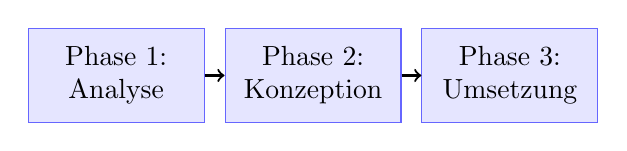
\begin{tikzpicture}[node distance=2.5cm, auto]
  % Boxen mit LIMAK-Farbe
  \node [rectangle, draw=blue!60, fill=blue!10, text width=2cm, text centered, minimum height=1.2cm] (phase1) {Phase 1:\\Analyse};
  \node [rectangle, draw=blue!60, fill=blue!10, text width=2cm, text centered, minimum height=1.2cm, right of=phase1] (phase2) {Phase 2:\\Konzeption};
  \node [rectangle, draw=blue!60, fill=blue!10, text width=2cm, text centered, minimum height=1.2cm, right of=phase2] (phase3) {Phase 3:\\Umsetzung};

  % Pfeile
  \draw[->, thick] (phase1) -- (phase2);
  \draw[->, thick] (phase2) -- (phase3);
\end{tikzpicture}
\caption{Beispielhafter Prozessablauf (eigene Darstellung)}
\label{fig:beispiel-prozess}
\end{figure}

\subsection{Implikationen für die Praxis}

Für die praktische Anwendung ergeben sich folgende Implikationen \parencite{Praktiker2022}:
\begin{itemize}
    \item {[Implikation 1]}
    \item {[Implikation 2]}
    \item {[Implikation 3]}
\end{itemize}

\section{[Theoriebereich 3 / Spezifisches Thema]}
\label{sec:theorie-bereich3}

%% Dieser Abschnitt kann für spezifischere Themen genutzt werden,
%% z.B. eine bestimmte Technologie, Methode oder Branche

\subsection{[Spezifisches Konzept]}

[Beschreibung des spezifischen Konzepts mit Bezug zu den vorherigen Abschnitten]

\subsection{Anwendung im Kontext von [Ihr Thema]}

Im Kontext von [Ihr Thema] ist [Konzept] besonders relevant, weil [Begründung]. Die Literatur zeigt, dass [wichtige Erkenntnisse für Ihr Thema] \parencite{RelevantAutor2023}.

\section{Synthese und Forschungslücke}
\label{sec:synthese}

%% Wichtig: Verbinden Sie die theoretischen Grundlagen mit Ihrer Forschungsfrage

Zusammenfassend lässt sich festhalten, dass die bisherige Forschung zu [Thema] wichtige Erkenntnisse in den Bereichen [Bereich 1] und [Bereich 2] geliefert hat. Allerdings zeigt sich eine Forschungslücke hinsichtlich [identifizierte Lücke].

Diese Arbeit adressiert diese Lücke, indem [Ihr Beitrag zur Schließung der Lücke]. Dabei wird auf die theoretischen Grundlagen aus den vorangegangenen Abschnitten aufgebaut, insbesondere auf [relevante Konzepte für Ihre Arbeit].
